\documentclass{beamer}

\setbeamertemplate{navigation symbols}{}
\usetheme{Montpellier}
\beamersetuncovermixins{\opaqueness<1>{25}}{\opaqueness<2->{15}}

\begin{document}
\title{Bayesian parameter synthesis of Markov population models.}
\author{Nhat-Huy Phung}

\begin{frame}
  \titlepage
\end{frame}

\begin{frame}
  \frametitle{Table of contents}
  \tableofcontents
\end{frame}

\section{Motivation}
\begin{frame}
  \frametitle{Motivation}
  %% Population process

\end{frame}

\section{Problem description}
\begin{frame}
  \frametitle{Markov population model}
  %% TODO: definition of markov population model
\end{frame}

\begin{frame}
  \frametitle{Parametric DTMC}
\end{frame}

\section{Model and properties}
\begin{frame}
  \frametitle{Approach}
  \begin{itemize}
    \item Model individual's behaviour as a Markov Decision Process.
    \item Model collective behaviour as a composition of many individual
          behavioural models.
    \item Answer the research question by checking the collective behaviour model
          against properties represented in the form of temporal logic.
  \end{itemize}
\end{frame}

\begin{frame}
  \frametitle{Single agent model.}
  We model the behaviour of a single bee as a Markov Decision Process. Let
  $\mathcal{S}$ be the individual model, we have
  \begin{align*}
    \mathcal{S} = (S, A, P_a, R_a)
  \end{align*}
  in which
  \begin{itemize}
    \item $S$ is the set of states.
    \item $A$ is the set of actions.
    \item $P_a(s,s')$ is the probability of transitioning from state $s$ to state
          $s'$ given action $a$.
    \item $R_a(s,s')$ is the \textit{reward} received after transitioning from
          state $s$ to state $s'$ given action $a$.
  \end{itemize}
\end{frame}

\begin{frame}
  \frametitle{Example model}
  Example of a single bee model
  %% TODO
\end{frame}

\begin{frame}
  \frametitle{Collective model}
  To model collective behavior of multiple agents, we construct product of
  individual models. Let $\mathcal{M}$ be the multiple agents model, we have
  \begin{align*}
    \mathcal{M} = (\mathcal{S}_1||\mathcal{S}_2||\ldots||\mathcal{S}_k)
  \end{align*}
  in which $k$ is the population size and $||$ denotes synchronous composition.\\
  As Markov Decision Process can be seen as a probabilistic automata,
  construction of MDPs composition follows [Sokolova].
\end{frame}

\begin{frame}
  \frametitle{Global properties}
  \textbf{Question:} How the aggressiveness of each individual at the beginning
  changes the population at the steady state.\\
  \textbf{Answer:} In our model, as each absorbing state represents a population
  size at the steady state, the question can be answered by checking the model
  against PCTL properties.
  \begin{align*}
    P_{?} (FG s_i)
  \end{align*}
  Where $s_i$ is the absorbing state represents the population size $i$ at the
  steady state. By parameter synthesis using synthetic data, we can observe how
  the synthetic model parameters change.
\end{frame}

\begin{frame}
  \frametitle{Global properties}
  \textbf{Question:} Is it always right, that the more individuals the colony
  has, the less aggressive each individual is?\\
  \textbf{Answer:} The approach to answer this question is to synthesize the
  model parameters for different population sizes and observe if the synthetic
  parameters shows that the more individuals a colony has, the less aggressive
  it will be.
\end{frame}

\begin{frame}
  \frametitle{Local properties}
  \textbf{Question:} Given a local PCTL property, for example, , synthesize the
  model
  parameters so that the property is satisfied. \\
  \textbf{Answer:} The approach to answer this question is to synthesize the
  model parameters by Bayesian parameter synthesis using synthetic data and then
  conclude
\end{frame}

\section{Framework}
\begin{frame}
  \frametitle{Proposed Framework}
  We propose a framework to synthesize model parameters based on the method
  presented in [Molyneux]
  \begin{figure}[t]
    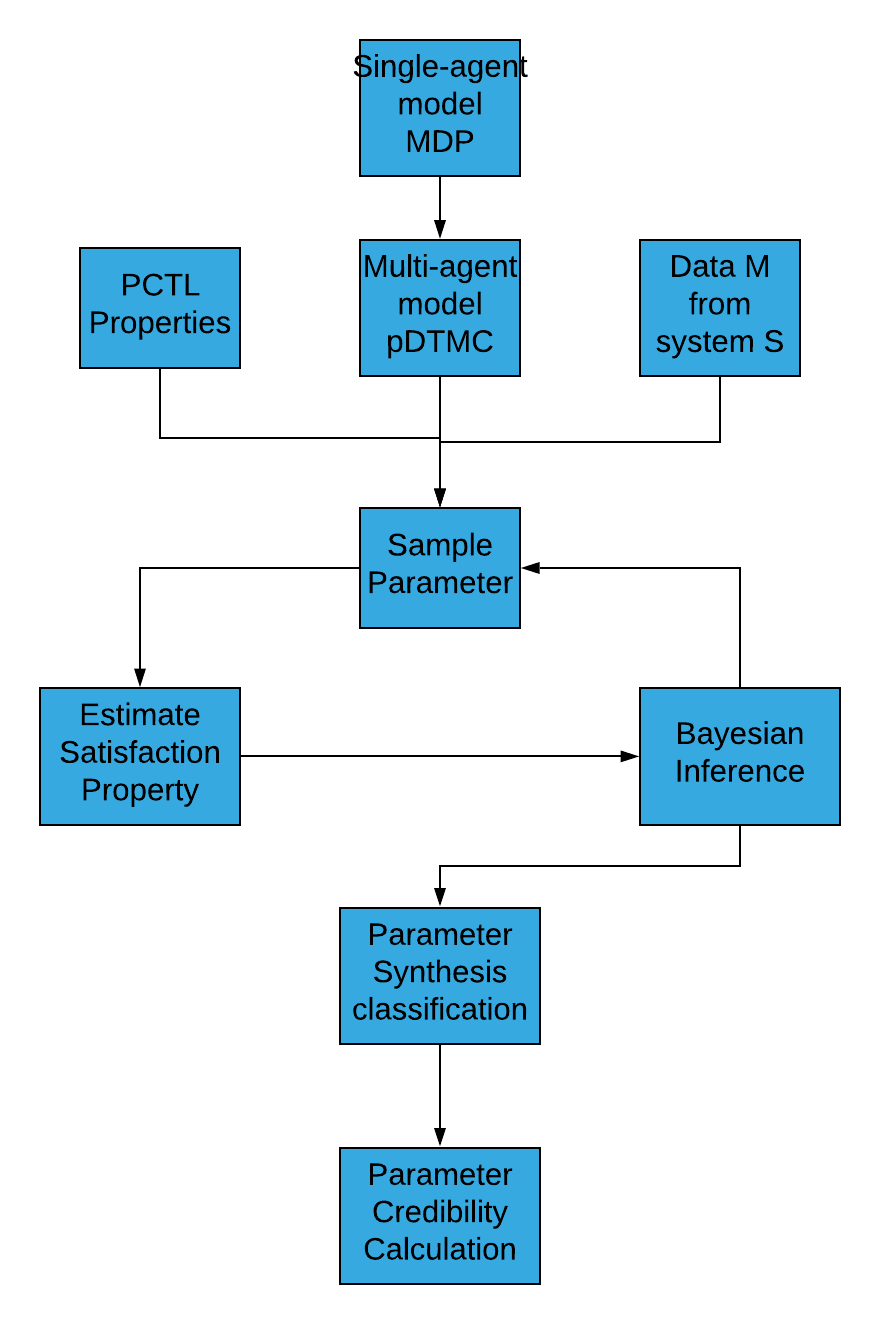
\includegraphics[height=\textheight]{abcsmc2.png} \centering
  \end{figure}
\end{frame}

\begin{frame}
  \frametitle{Tools}
  For probabilistic model checking and parameter synthesis, we use STORM
  probabilisttic model checker
  \begin{itemize}
    \item Faster, compare to PRISM.
    \item Stronger symbolic algebra engine: STORM is capable of delivering more
          compact symbolic results.
    \item Provides better APIs (PRISM has no API for )
  \end{itemize}
\end{frame}

\section{Case study}
\begin{frame}
  \frametitle{Case study}
  We study the defensive behaviour of a bee colony.
  \begin{itemize}
    \item Bees response to stimulations from the environment by \textit{stinging}.
    \item After \textit{stinging}, an individual bee releases \textit{pheromone}
          and dies.
  \end{itemize}
  Our questions concerns the relation between the concentration of pheromone in
  the environment and the aggressiveness of each individual in the colony.
\end{frame}

\begin{frame}
  \frametitle{Case study}
  As we study the biological system, we have the following research questions:
  \begin{enumerate}
    \item Given a population of bee, how many individuals left in the steady
          state.
    \item How does an individual's behaviour change the collective behaviour? Does
          each individual become more aggresive given the
  \end{enumerate}
  The purpose of this thesis is to study these questions using probabilistic
  modeling and model checking.\\
  In the scope of this thesis we use bees colony as a case study. However, the
  method can be applied to general parametric Discrete-Time Markov Chain models.
\end{frame}

\begin{frame}
  \frametitle{Data}
  \begin{itemize}
    \item \textbf{Biological data} is collected from a real bee colony, which is
          currently maintained by Department of Biology.
    \item \textbf{Synthetic data} is generated by simulating the parametric DTMC
          using a concrete assignment of parameters.
  \end{itemize}
  Using \textit{synthetic data} has an advantage over using real data. Namely,
  as the concrete parameters are known, it is possible to measure the distance
  between the synthesized parameters and true parameters.
\end{frame}
\section{Case study}
\begin{frame}
  \frametitle{Case study}
  We study the defensive behaviour of a bee colony.
  \begin{itemize}
    \item Bees response to stimulations from the environment by \textit{stinging}.
    \item After \textit{stinging}, an individual bee releases \textit{pheromone}
          and dies.
  \end{itemize}
  Our questions concerns the relation between the concentration of pheromone in
  the environment and the aggressiveness of each individual in the colony.
\end{frame}

\begin{frame}
  \frametitle{Case study}
  As we study the biological system, we have the following research questions:
  \begin{enumerate}
    \item Given a population of bee, how many individuals left in the steady
          state.
    \item How does an individual's behaviour change the collective behaviour? Does
          each individual become more aggresive given the
  \end{enumerate}
  The purpose of this thesis is to study these questions using probabilistic
  modeling and model checking.\\
  In the scope of this thesis we use bees colony as a case study. However, the
  method can be applied to general parametric Discrete-Time Markov Chain models.
\end{frame}

\begin{frame}
  \frametitle{Data}
  \begin{itemize}
    \item \textbf{Biological data} is collected from a real bee colony, which is
          currently maintained by Department of Biology.
    \item \textbf{Synthetic data} is generated by simulating the parametric DTMC
          using a concrete assignment of parameters.
  \end{itemize}
  Using \textit{synthetic data} has an advantage over using real data. Namely,
  as the concrete parameters are known, it is possible to measure the distance
  between the synthesized parameters and true parameters.
\end{frame}

\section{Timeline}
\begin{frame}
  \frametitle{Timeline}
  Thesis milestones
  \begin{enumerate}
    \item \textbf{25.11.2020}: Model and properties lists.
    \item \textbf{10.12.2020}: Framework implementation and results.
    \item \textbf{30.01.2021}: Thesis submission.
  \end{enumerate}
  Progress is reported weekly.
\end{frame}

\end{document}
